%!TEX root = ..\arxiv_Dampinguncertanity_manuscript.tex
%-------------------------------
%*******************************
\section{UNCERTAINTY ANALYSIS}
\label{sec:method}

In this section, we perform the uncertainty analysis on the areas approach~\cite{Huang2007} to identify the structural damping ratio. 
We develop guidelines for an optimal number of areas to be considered for accurate damping estimation. This method yields precise estimate of the damping ratio with noise, even for a higher damping ratio($\xi$).

We define the areas logarithmic decrement ratio as
\begin{equation}
\delta_{\rm A}=\ln \frac{A_{1}}{A_{n+1}}=\ln \frac{A \mathrm{e}^{-\xi \omega_{n} t_{i}}}{A \mathrm{e}^{-\xi \omega_{n}\left(t_{i}+n T_{d}\right)}}=\xi \omega_{n} T_{d} n=\frac{2 n \pi \xi}{\sqrt{1-\xi^{2}}},
\end{equation}
where $T_d$ is damped time period, $\omega_{n}$ is the natural frequency, $n$ number of periods and $A$ is the amplitude of the signal.
\begin{figure}[h]
\label{sin}
\includegraphics[scale=0.25]{sinwave_area}
\centering
\caption{The free decay response of the signal.}
\end{figure}

Next, we define $S_{1}, \ldots, S_{N}$ (see Fig.~\ref{sin}) as the areas corresponding to the zero-crossings of the signal. 
For example, the expressions for the two first areas are given by 
\begin{equation}
\label{e9}
\begin{aligned}
&S_{1}=\int_{t_{1}}^{t_{1}+\frac{T_{d}}{2}}|x(t)| \mathrm{d} t=\int_{0}^{\frac{T_{d}}{2}}\left|x\left(t+t_{1}\right)\right| \mathrm{d} t\\
&=A \mathrm{e}^{-\xi \omega_{n} t_{1}} \int_{0}^{\frac{T_{d}}{2}}\left|\mathrm{e}^{-\xi \omega_{n} t} \sin \left(\omega_{d} t+\varphi+\omega_{d} t_{1}\right)\right| \mathrm{d} t\\
&S_{2}=\int_{t_{1}+\frac{T_{d}}{2}}^{t_{1}+T_{d}}|x(t)| \mathrm{d} t=\int_{0}^{\frac{T_{d}}{2}}\left|x\left(t+t_{1}+\frac{T_{d}}{2}\right)\right| \mathrm{d} t\\
&=A \mathrm{e}^{-\xi \omega_{n} t_{1}} \mathrm{e}^{-\xi \omega_{n} \frac{T_{d}}{2}} \int_{0}^{\frac{T_{d}}{2}}\left|\mathrm{e}^{-\xi \omega_{n} t} \sin \left(\omega_{d} t+\varphi+\omega_{d} t_{1}\right)\right| \mathrm{d} t.
\end{aligned}
\end{equation}

The relationship between areas can be obtained from Eq.~\eqref{e9} as
\begin{equation}
\label{e1}
S_{2}=S_{1} \mathrm{e}^{-\xi \omega_{n} \frac{T_{d}}{2}}.
\end{equation}
Similarly one can obtain
\begin{equation}
\label{e2}
S_{2 N}=S_{2 N-1} \mathrm{e}^{-\xi \omega_{n} \frac{T_{d}}{2}}.
\end{equation}
The expression for $\xi$ in terms of $S_{1}..S_{N}$, can be obtained as follows
\begin{equation}
\label{eq1}
\begin{aligned}
&\frac{S_{1}+S_{2}+\cdots+S_{N}}{S_{N+1}+S_{N+2}+\cdots+S_{2 N}}=\frac{S_{1}+S_{2}+\cdots+S_{N}}{\left(S_{1}+S_{2}+\cdots+S_{N}\right) \mathrm{e}^{-\xi \omega_{n} n T_{d}/2}}\\ &=\mathrm{e}^{\xi \omega_{n} n T_{d}/2}=\mathrm{e}^{ n \pi \xi} / \sqrt{1-\xi^{2}}.
\end{aligned}
\end{equation}
From Eq.~\eqref{eq1} damping ratio $\xi$ is
\begin{equation}
\xi=1 / \sqrt{1+\left(n \frac{\pi}{E}\right)^{2}},
\end{equation}
where $E=\ln \left(\sum S_{k} / \sum S_{k+N}\right)$, which is the natural logarithm of the ratio of summation of the former $N$ areas to the summation of the latter $N$ areas.


From equations Eqs.\eqref{e1} and \eqref{e2} we can write

\begin{equation}
\begin{array}{c}

S_{2}=S_{1}\epsilon\\
S_{3}=S_{1} \epsilon^{2} \\
\vdots \\
S_{N}=S_{1} \epsilon^{N-1}
\end{array}
\end{equation}
where $ \epsilon=\mathrm{e}^{-\xi \omega_{n} \frac{T_{d}}{2}}.$

The summation of first $N$ areas in Eq.~\eqref{eq1} is given by
\begin{equation}
\begin{aligned}
U_N=S_{1}+S_{2}+\cdots+S_{N}=S_1 (1+\epsilon+\epsilon^2+\epsilon^3\cdots\epsilon^{N-1}).
\end{aligned}
\end{equation}
Differentiating $U_N$ with respect to $\xi$ gives
% \begin{equation}
\begin{align}
\frac{\partial U_N}{\partial \xi}&=S_{1}(0+c\epsilon+2c\epsilon^2+3c\epsilon^3\cdots(N-1)c\epsilon^{N-1}), \nonumber\\
                                 &=S_{1}c\epsilon(1+2\epsilon+3\epsilon^2+\cdots+(N-1)\epsilon^{N-2})  
\label{e3}
\end{align}
% \end{equation}

% \begin{equation}
% \label{e3}
% \frac{\partial U_N}{\partial \xi}=S_{1}c\epsilon(1+2\epsilon+3\epsilon^2\cdots(N-1)\epsilon^{N-2}),
% \end{equation}
where $c=-\omega_{n} \frac{T_{d}}{2}$.\\
Eq.~\eqref{e3} is an arithmetic geometric progression, with $\mid \epsilon \mid \leq 1 $. 
The sum of terms of the progression is given by
\begin{equation}
\label{e6}
\frac{\partial U_N}{\partial \xi}=S_{1}c\epsilon\left[\frac{1-N \epsilon^{N-1}}{1-\epsilon}+\frac{\epsilon \left(1-\epsilon^{N-1}\right)}{(1-\epsilon)^{2}}\right].
\end{equation}
Similarly, we can write the summation of the subsequent $N$ areas in Eq.\eqref{eq1} as
\begin{equation}
\begin{aligned}
U_D&=S_{N+1}+S_{N+2}+\cdots+S_{2N}\\
&=S_1 \epsilon^N(1+\epsilon+\epsilon^2+\epsilon^3\cdots\epsilon^{N-1}).
\end{aligned}
\end{equation}
Differentiating $U_D$ with respect to $\xi$ gives
\begin{multline}
\label{e7}
\frac{\partial U_D}{\partial \xi}=S_{1}N c \epsilon^N(1+\epsilon+\epsilon^2+\epsilon^3\cdots\epsilon^{N-1})\\
+S_1 \epsilon^N(0+c\epsilon+2c\epsilon^2+3c\epsilon^3\cdots(N-1)c\epsilon^{N-1}).
\end{multline}

In Eq.~\eqref{e7}, we notice that the first term is a geometric series, and the second term is an arithmetic geometric progression with $\mid \epsilon \mid \leq 1 $. 
The sum of the terms then becomes
\begin{multline}
\label{equd}
\frac{\partial U_D}{\partial \xi}=S_{1}N c \epsilon^N \left(\frac{1-\epsilon^{N}}{1-\epsilon}\right)\\
+S_1c \epsilon^{N+1}\left[\frac{1-N \epsilon^{N-1}}{1-\epsilon}+\frac{\epsilon \left(1-\epsilon^{N-1}\right)}{(1-\epsilon)^{2}}\right].
\end{multline}

The total uncertainty in Eq.\eqref{eq1} is given by
\begin{equation}
\label{equn}
U^2_{\xi}=\left[\left(\frac{\partial U_{N}}{\partial \xi}\right)^{2}+\left(\frac{\partial U_{D}}{\partial \xi}\right)^{2}\right]U_x^2,
\end{equation}
where $U_x$ is the uncertainty in measuring the response. 
Substituting Eqs.~\eqref{e6}~and~\eqref{equd} into Eq.~\eqref{equn} gives
\begin{equation}
\label{tuc}
\begin{array}{l}
U_{\xi}^{2}=\left\{\left(S_{1} c \varepsilon\left[\frac{1-N \varepsilon^{N-1}}{1-\varepsilon}+\frac{\varepsilon\left(1-\varepsilon^{N-1}\right)}{(1-\varepsilon)^{2}}\right]\right)^{2}\right. \\
\left.+\left(S_{1} N c \varepsilon^{N}\left(\frac{1-\varepsilon^{N}}{1-\varepsilon}\right)+S_{1} c \varepsilon^{N+1}\left[\frac{1-N \varepsilon^{N-1}}{1-\varepsilon}+\frac{\varepsilon\left(1-\varepsilon^{N-1}\right)}{(1-\varepsilon)^{2}}\right]\right)^{2}\right\}U_x^2
\end{array}
\end{equation}

\begin{figure}[h]

\centering
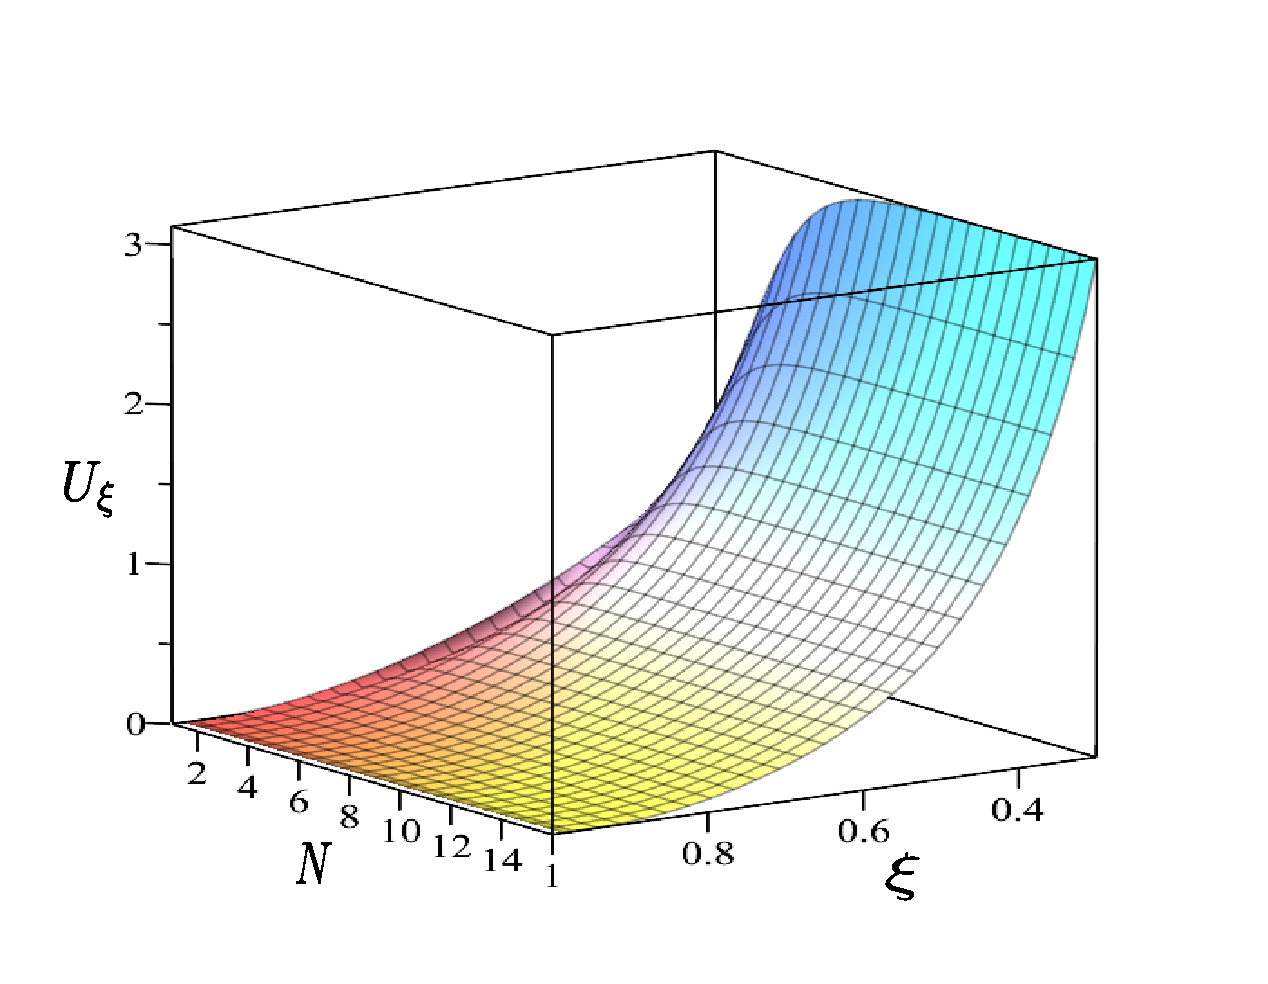
\includegraphics[scale=0.45]{Surf1uz0p3}

\caption{The variation of uncertainty ($U_{\xi}$) with $N$ and $\xi$.}
\label{4}


\end{figure}

Figure~\ref{4} shows the uncertainty $U_{\xi}$ variation with $N$ and $\xi$, we can observe that as $\xi$ decreases and $N$ increases, the uncertainty will be maximum.

Our goal is to find out the optimal number of areas to minimize the uncertainty in predicted damping ratio $\xi$. Which can be achieved by differentiating $U_\xi$ with respect $N$ and solving for $N$.
Differentiating Eq.~\eqref{tuc} with respect to $N$ yields
\begin{equation}
\label{e10}
\begin{aligned}
&\frac{\partial U_{\xi}}{\partial N}=\left\{2 S_1^{2} c^{2} \epsilon^{2}\left(\frac{1-N \epsilon^{N-1}}{1-\epsilon}+\frac{\epsilon\left(1-\epsilon^{N-1}\right)}{(1-\epsilon)^{2}}\right)\right. \\
&\left(\frac{-\epsilon^{N-1}-N \epsilon^{N-1} \ln (\epsilon)}{1-\epsilon}-\frac{\epsilon \epsilon^{N-1} \ln (\epsilon)}{(1-\epsilon)^{2}}\right)\\
&+2\left(\frac{S_1 N c \epsilon^{N}\left(1-\epsilon^{N}\right)}{1-\epsilon}+S_1 c \epsilon^{N+1}\left(\frac{1-N \epsilon^{N-1}}{1-\epsilon}+\frac{\epsilon\left(1-\epsilon^{N-1}\right)}{(1-\epsilon)^{2}}\right)\right) \\
&\left(\frac{S_1 c \epsilon^{N}\left(1-\epsilon^{N}\right)}{1-\epsilon}+\frac{S_1 N c \epsilon^{N} \ln (\epsilon)\left(1-\epsilon^{N}\right)}{1-\epsilon}-\frac{S_1 N c\left(\epsilon^{N}\right)^{2} \ln (\epsilon)}{1-\epsilon}\right. \\
&\left.+S_1 c \epsilon^{N+1} \ln (\epsilon)\left(\frac{1-N \epsilon^{N-1}}{1-\epsilon}+\frac{\epsilon\left(1-\epsilon^{N-1}\right)}{(1-\epsilon)^{2}}\right)\right. \\
&\left.+S_1 c \epsilon^{N+1}\left(\frac{-\epsilon^{N-1}-N \epsilon^{N-1} \ln (\epsilon)}{1-\epsilon}-\frac{\epsilon \epsilon^{N-1} \ln (\epsilon)}{(1-\epsilon)^{2}}\right)\right\}\frac{ U_{x}}{2U_{\xi}}.
\end{aligned}
\end{equation}

Equation~\eqref{e10} does not have have a closed form solution for $N \geq 2$; therefore, we must use numerical solutions to obtain the optimal $N$. 
Note that we assume that $S_1=1$, i.e., we do not consider uncertainties in the zero-crossings in our analysis. The uncertainty in measurement($U_x$) will not affect the optimal number areas since it is constant.
\begin{figure}[h]
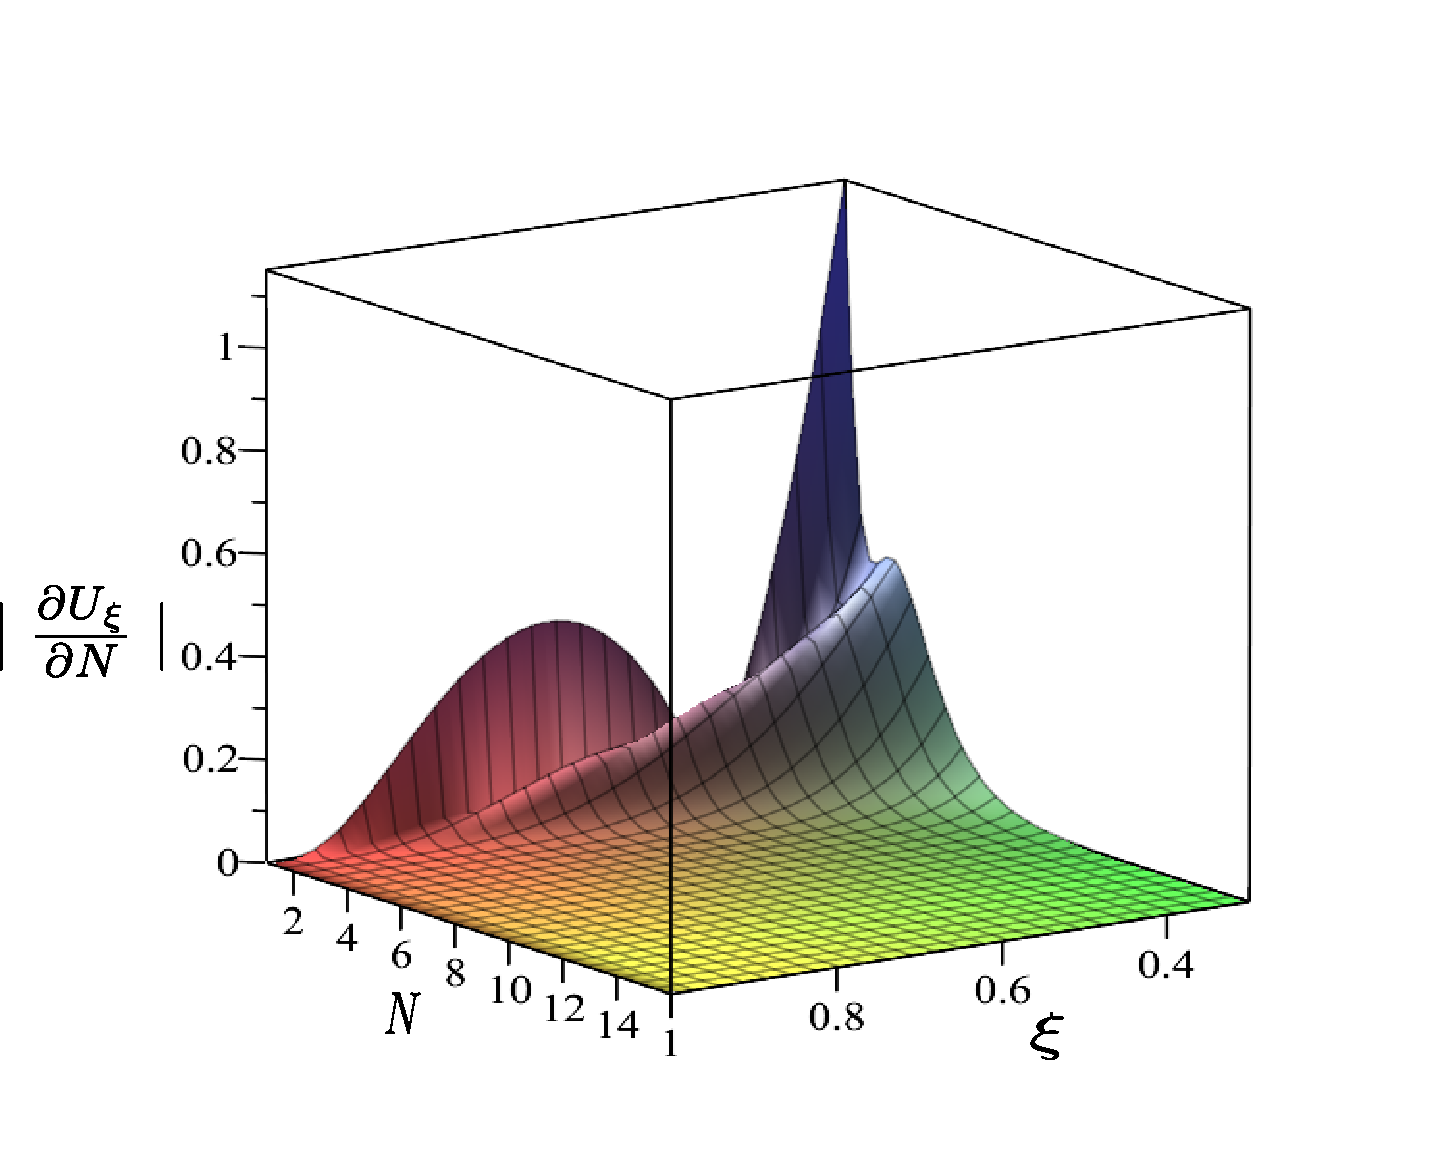
\includegraphics[scale=0.4]{Surf1z0p3}
\centering
\caption{The variation of rate of uncertainty with $N$ for high damping ratio($\xi$).}
\label{uH}
\end{figure}
\begin{figure}[h]
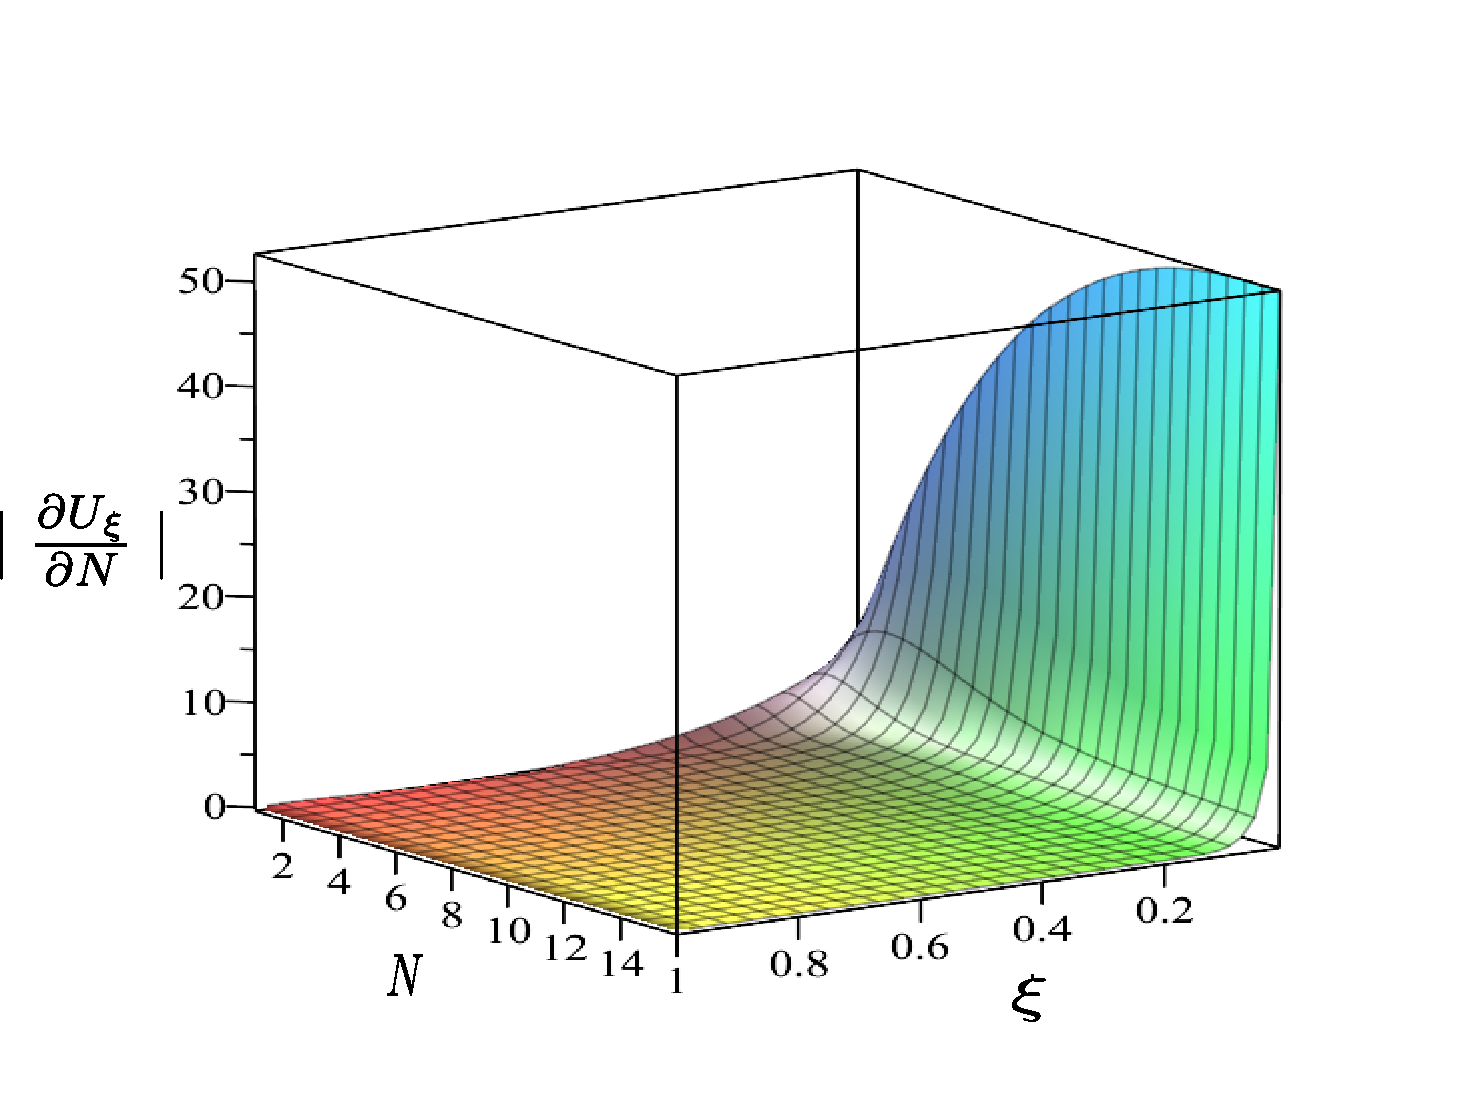
\includegraphics[scale=0.4]{Surf1z0p1}
\centering
\caption{The variation of rate of uncertainty with $N$ and for low to high damping ratio($\xi$).}
\label{uL}
\end{figure}

\begin{figure}[h]
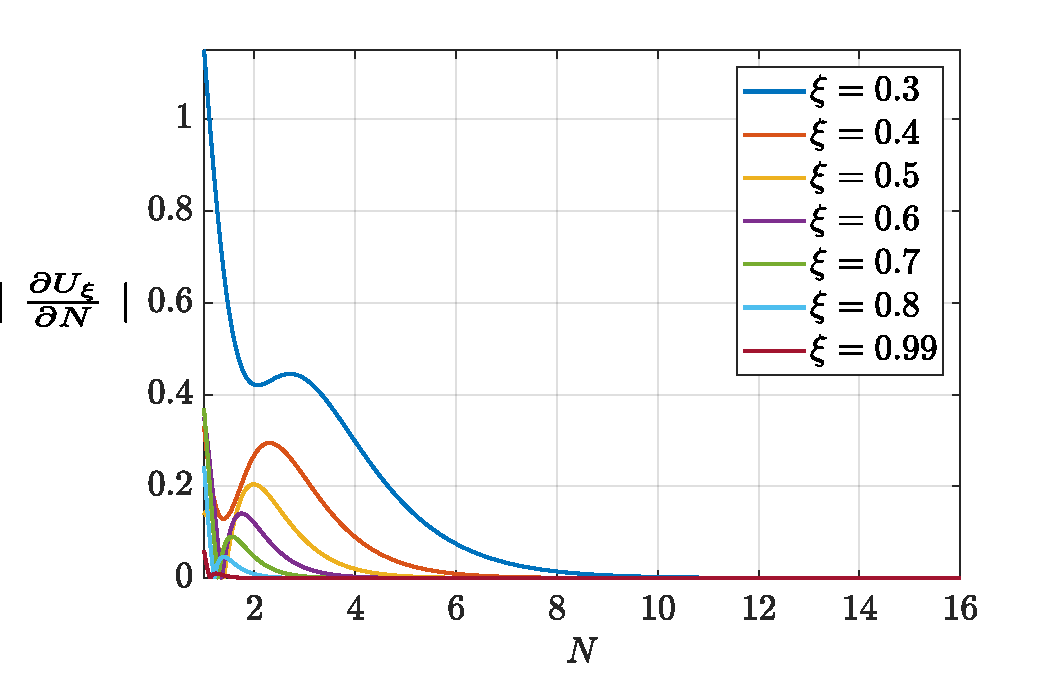
\includegraphics[scale=0.5]{zN}
\centering
\caption{The variation of rate of uncertainty with $N$ for high damping ratio($\xi$).}
\label{uH1}
\end{figure}
\begin{figure}[h]
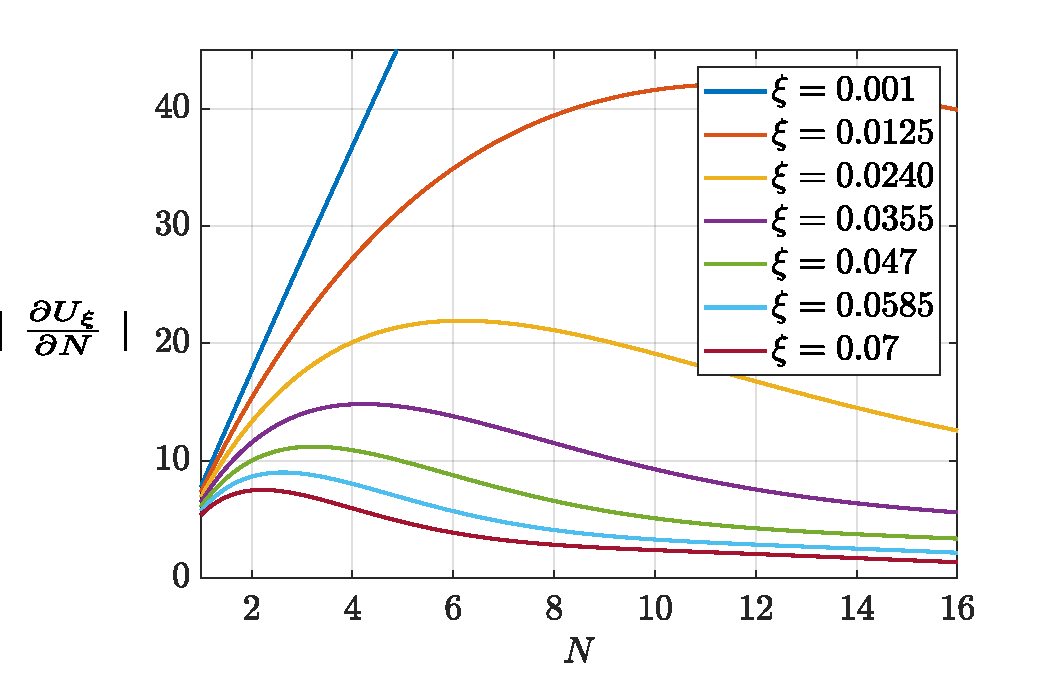
\includegraphics[scale=0.5]{zN1}
\centering
\caption{The variation of rate of uncertainty with $N$ for very low damping ratio($\xi$).}
\label{uL1}
\end{figure}

From Figs.~\ref{uH} and \ref{uH1}, we can observe that for high damping ratios, we see a local maximum in the rate of uncertainty with N. We can also observe that the uncertainty decreases as $N$ increases. Based on these observations, we can say that for a high damping ratio $\xi$, consider as many areas as possible and avoid picking up $N$, which is at local maxima to minimize the error in predicted $\xi$.
For a very low damping ratio, from Fig.~\ref{uL1} we can see that the rate of uncertainty increases enormously as we raise $N$ for very low damping we need to consider as minimum areas as possible to minimize the error in predicted $\xi$.
%%%%%%%%%%%%%%%%
%%%%%%%%%%%%%%%%

